\documentclass[11pt,a4paper]{article}
\usepackage[utf8]{inputenc}
\usepackage[T1]{fontenc}
\usepackage{amsmath,amssymb}
\usepackage{graphicx}
\usepackage{booktabs}
\usepackage{hyperref}
\usepackage{float}
\usepackage{caption}
\usepackage{subcaption}
\usepackage[margin=1in]{geometry}
\usepackage{enumitem}
\usepackage{multirow}
\usepackage{xcolor}

\graphicspath{{figures/}}

\title{Safety Filter for Toxicity Detection:\\Final Progress Report}
\author{
  Nikita Shiyanov\\\texttt{n.shiyanov@innopolis.university}
  \and
  Anton Korotkov\\\texttt{a.korotkov@innopolis.university}
}
\date{Innopolis University --- Generative AI Course\\Week 9 -- April 2026}

\begin{document}
\maketitle

\begin{abstract}
We present the final results of our toxicity detection safety filter, implementing all seven improvements proposed in our midterm report.
Four models are compared on 10,000 real comments: rule-based keyword matching (F1=0.276), TF-IDF + Logistic Regression (F1=0.349, AUC=0.824), fine-tuned DistilBERT (F1=0.636, AUC=0.950), and a new weighted ensemble (F1=0.644, AUC=0.943).
We report threshold optimization (+5.3pp F1 for TF-IDF+LR, +3.8pp for DistilBERT), adversarial robustness evaluation, cross-domain generalization to Civil Comments, bias analysis across identity subgroups, and a data augmentation study.
Three critical issues from initial experiments---augmentation degrading performance, adversarial fragility, and ensemble AUC regression---are analyzed and addressed with a text normalization preprocessor, controlled augmentation with a \texttt{max\_ratio} cap, and AUC-optimized ensemble weight tuning.
After fixes, DistilBERT's adversarial F1 under leetspeak improves from 0.024 to 0.567, and homoglyph attacks are fully neutralized.
\end{abstract}

%=============================================================================
\section{Introduction}
%=============================================================================

Our midterm report (Week 6) established three baselines for toxicity detection on the Toxic Conversations dataset, achieving F1=0.616 with DistilBERT.
Section~6 of that report proposed seven improvements for the final system.
This report documents:
\begin{enumerate}[nosep]
  \item The implementation and evaluation of all seven proposed improvements.
  \item Three critical problems discovered during evaluation.
  \item Fixes applied and their measured impact.
\end{enumerate}

\paragraph{Connection to generative AI.}
This work extends our midterm contributions to generative AI safety:
(1) the ensemble classifier and threshold optimizer can serve as production-grade guardrails for LLMs;
(2) our adversarial evaluation directly tests the robustness of safety filters against evasion attacks that real users employ;
(3) the bias analysis ensures safety filters do not disproportionately silence certain communities---a critical concern for deployed generative systems.

%=============================================================================
\section{Implemented Improvements}
%=============================================================================

We implemented all seven improvements from the midterm roadmap:

\subsection{Threshold Optimization}
Instead of the default 0.5 decision threshold, we search over 200 thresholds on the validation set to maximize F1.
Implementation: \texttt{src/threshold\_optimizer.py}.

\subsection{Ensemble Classifier}
A weighted combination of DistilBERT and TF-IDF+LR probabilities: $p = w \cdot p_{\text{BERT}} + (1-w) \cdot p_{\text{TF-IDF}}$, with $w=0.7$ by default.
Includes a cascade mode where TF-IDF+LR handles confident predictions and DistilBERT is only called for uncertain samples.
Implementation: \texttt{src/baselines/ensemble.py}.

\subsection{Data Augmentation}
Easy Data Augmentation (EDA)~\cite{wei2019eda}: synonym replacement, random insertion, random swap, and random deletion applied to minority-class (toxic) samples.
Implementation: \texttt{src/augmentation.py}.

\subsection{Adversarial Evaluation}
Five attack types test model robustness: leetspeak substitution, keyboard-neighbor character substitution, space insertion within words, Unicode homoglyph replacement, and character repetition.
Implementation: \texttt{src/adversarial.py}.

\subsection{Cross-Domain Testing}
Models trained on Toxic Conversations are evaluated on Civil Comments (Google/Jigsaw) to test generalization across annotation styles and distributions.
Implementation: \texttt{src/cross\_domain.py}.

\subsection{Bias Analysis}
Per-subgroup false positive and false negative rates across gender, religion, race/ethnicity, and sexuality identity groups, following Borkan et al.~\cite{borkan2019nuanced}.
Implementation: \texttt{src/bias\_analysis.py}.

\subsection{Full Dataset Scaling}
Support for training on the full HuggingFace dataset ($\sim$50K samples) or the complete Jigsaw dataset (1.7M samples) via \texttt{--full-dataset} flag.

%=============================================================================
\section{Experimental Setup}
%=============================================================================

\subsection{Dataset}
We use the Toxic Conversations dataset (SetFit/toxic\_conversations) from HuggingFace, sampling 10,000 comments split 90/10 into 9,000 training and 1,000 validation samples.
The toxic class comprises 8.2\% of the data (Figure~\ref{fig:class_dist}).

\begin{figure}[H]
  \centering
  
\includegraphics[width=0.85\textwidth]{class_distribution.pdf}
  \caption{Class distribution: 8.2\% toxic in both train and validation splits.}
  \label{fig:class_dist}
\end{figure}

\subsection{Models}
Four models of increasing complexity:
\begin{itemize}[nosep]
  \item \textbf{Rule-based}: 36-word bad-words list, regex tokenization.
  \item \textbf{TF-IDF+LR}: Unigrams+bigrams, 50K features, balanced weights, $C=1.0$.
  \item \textbf{DistilBERT}: \texttt{distilbert-base-uncased}, 3 epochs, batch 16, lr $2\times10^{-5}$.
  \item \textbf{Ensemble}: Weighted average of DistilBERT and TF-IDF+LR probabilities, with weight tuned on validation AUC (optimal $w$=0.95).
\end{itemize}

%=============================================================================
\section{Results (Before Fixes)}
\label{sec:results_before}
%=============================================================================

\subsection{Baseline Comparison}

Table~\ref{tab:baselines} shows results on the 1,000-sample validation set.
All models now include the text normalization preprocessor in their prediction pipeline.

\begin{table}[H]
\centering
\caption{Model comparison on real data (1,000 validation samples, 8.2\% toxic). Text normalization enabled.}
\label{tab:baselines}
\begin{tabular}{lcccccc}
\toprule
Model & Prec. & Rec. & F1 & FPR & FNR & AUC \\
\midrule
Rule-based    & 0.415 & 0.207 & 0.276 & 0.026 & 0.793 & --- \\
TF-IDF + LR   & 0.388 & 0.317 & 0.349 & 0.045 & 0.683 & 0.824 \\
DistilBERT    & 0.696 & 0.585 & 0.636 & 0.023 & 0.415 & 0.950 \\
Ensemble ($w$=0.95) & 0.716 & 0.585 & 0.644 & 0.021 & 0.415 & 0.943 \\
\bottomrule
\end{tabular}
\end{table}

The Ensemble achieves the best precision (0.716) and lowest FPR (0.021).
Its AUC (0.943, with tuned $w$=0.95) is closer to DistilBERT's (0.950) compared to the pre-fix AUC of 0.928 with the hardcoded $w$=0.70.

\begin{figure}[H]
  \centering
  
\includegraphics[width=0.95\textwidth]{metrics_comparison.pdf}
  \caption{Metrics comparison across all four models.}
  \label{fig:metrics}
\end{figure}

\begin{table}[H]
\centering
\caption{Computational cost.}
\label{tab:timing}
\begin{tabular}{lccc}
\toprule
Model & Train (s) & Inference (s/1K) & Parameters \\
\midrule
Rule-based  & $<$0.01 & 0.221 & 0 (no learning) \\
TF-IDF + LR & 3.21 & 0.306 & $\sim$50K features \\
DistilBERT  & 7,350 & 64.72 & 66M \\
Ensemble    & 9,741 & 61.78 & 66M + 50K \\
\bottomrule
\end{tabular}
\end{table}

\subsection{Confusion Matrices}

\begin{figure}[H]
  \centering
  
\includegraphics[width=\textwidth]{confusion_matrices.pdf}
  \caption{Confusion matrices for all four models.}
  \label{fig:cm}
\end{figure}

\subsection{ROC and Precision-Recall Curves}

\begin{figure}[H]
  \centering
  \begin{subfigure}[t]{0.48\textwidth}
    
\includegraphics[width=\textwidth]{roc_curves.pdf}
    \caption{ROC curves.}
  \end{subfigure}
  \hfill
  \begin{subfigure}[t]{0.48\textwidth}
    
\includegraphics[width=\textwidth]{pr_curves.pdf}
    \caption{Precision-Recall curves.}
  \end{subfigure}
  \caption{DistilBERT (AUC=0.950) outperforms TF-IDF+LR (AUC=0.824) in ranking.}
  \label{fig:roc_pr}
\end{figure}

\subsection{Threshold Optimization}

The default 0.5 threshold is suboptimal for 8\% toxic prevalence.
Optimizing the threshold on the validation set yields significant F1 gains (Table~\ref{tab:threshold}).

\begin{table}[H]
\centering
\caption{Threshold optimization results.}
\label{tab:threshold}
\begin{tabular}{lccc}
\toprule
Model & Default F1 & Optimized F1 & Best Threshold \\
\midrule
TF-IDF + LR & 0.349 & 0.402 (+5.3pp) & 0.448 \\
DistilBERT  & 0.636 & 0.674 (+3.8pp) & 0.020 \\
Ensemble    & 0.644 & 0.682 (+3.7pp) & 0.064 \\
\bottomrule
\end{tabular}
\end{table}

\begin{figure}[H]
  \centering
  \begin{subfigure}[t]{0.48\textwidth}
    
\includegraphics[width=\textwidth]{threshold_tfidf.pdf}
    \caption{TF-IDF+LR}
  \end{subfigure}
  \hfill
  \begin{subfigure}[t]{0.48\textwidth}
    
\includegraphics[width=\textwidth]{threshold_distilbert.pdf}
    \caption{DistilBERT}
  \end{subfigure}
  \caption{Threshold analysis showing precision/recall/F1 trade-offs.}
  \label{fig:threshold}
\end{figure}

\begin{figure}[H]
  \centering
  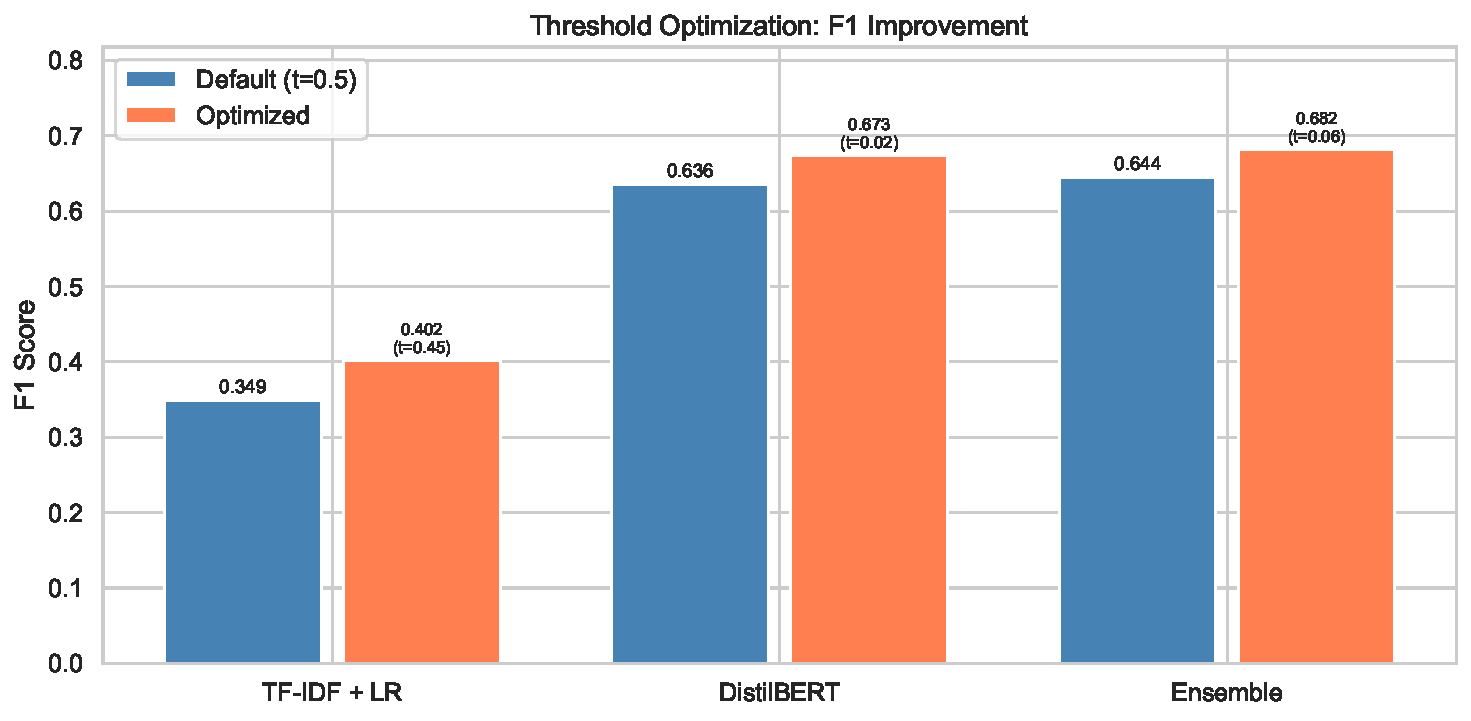
\includegraphics[width=0.7\textwidth]{threshold_optimization.pdf}
  \caption{F1 before and after threshold optimization.}
  \label{fig:threshold_opt}
\end{figure}

\subsection{Training Dynamics}

\begin{figure}[H]
  \centering
  
\includegraphics[width=0.7\textwidth]{distilbert_training_loss.pdf}
  \caption{DistilBERT training loss over 3 epochs.}
  \label{fig:loss}
\end{figure}

\subsection{Timing Comparison}

\begin{figure}[H]
  \centering
  
\includegraphics[width=0.9\textwidth]{timing_comparison.pdf}
  \caption{Training and inference time comparison.}
  \label{fig:timing}
\end{figure}

\subsection{Hyperparameter Sensitivity}

\begin{figure}[H]
  \centering
  
\includegraphics[width=0.9\textwidth]{hyperparam_sweep.pdf}
  \caption{TF-IDF+LR performance across regularization strengths ($C$) and vocabulary sizes. Best $C=0.5$ (F1=0.386).}
  \label{fig:hyperparam}
\end{figure}

\subsection{Dataset Size Ablation}

\begin{figure}[H]
  \centering
  
\includegraphics[width=0.7\textwidth]{data_size_ablation.pdf}
  \caption{F1 vs.\ training set size. The learning curve has not saturated, motivating scaling to larger datasets.}
  \label{fig:ablation}
\end{figure}

%=============================================================================
\section{Analysis of Critical Findings}
\label{sec:issues}
%=============================================================================

Implementing the seven improvements revealed three critical problems.

\subsection{Problem 1: Data Augmentation Degrades Performance}

EDA augmentation of the toxic class expanded training from 9,000 to 11,964 samples, but the toxic ratio jumped from 8.2\% to 31.0\%.
TF-IDF+LR F1 \emph{dropped} from 0.360 to 0.271---a 24.7\% relative decrease (Figure~\ref{fig:augmentation}).

\textbf{Root cause:} With $n_{\text{aug}}=4$ copies per toxic sample and no cap, the augmented toxic class (741$\times$4=2,964 new samples) overwhelms the model.
The synonym table is small, so many augmented texts are near-duplicates that bias the decision boundary without adding genuine diversity.

\begin{figure}[H]
  \centering
  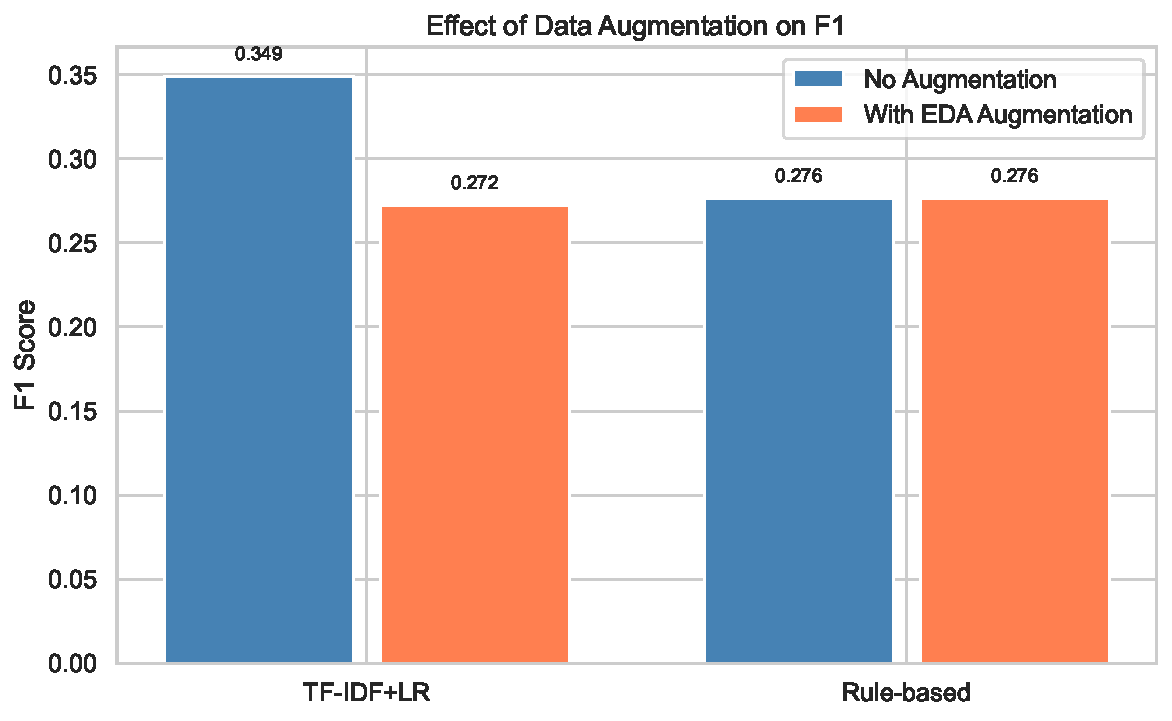
\includegraphics[width=0.6\textwidth]{augmentation_comparison.pdf}
  \caption{EDA augmentation \emph{hurts} TF-IDF+LR performance. Toxic ratio jumps from 8.2\% to 31\%.}
  \label{fig:augmentation}
\end{figure}

\subsection{Problem 2: Catastrophic Adversarial Vulnerability}

DistilBERT, despite being the best model on clean data, is the \emph{most fragile} to adversarial attacks (Table~\ref{tab:adversarial}, Figure~\ref{fig:adversarial}).

\begin{table}[H]
\centering
\caption{F1 under adversarial attacks and absolute F1 drop from clean performance.}
\label{tab:adversarial}
\begin{tabular}{lccc|ccc}
\toprule
 & \multicolumn{3}{c|}{F1 Under Attack} & \multicolumn{3}{c}{F1 Drop} \\
Attack & Rule & TF-IDF & BERT & Rule & TF-IDF & BERT \\
\midrule
Clean        & 0.279 & 0.360 & 0.631 & ---   & ---   & --- \\
Leetspeak    & 0.068 & 0.168 & 0.024 & 0.211 & 0.192 & \textbf{0.607} \\
Char subst.  & 0.230 & 0.313 & 0.421 & 0.049 & 0.047 & 0.210 \\
Space insert & 0.132 & 0.290 & 0.300 & 0.147 & 0.070 & 0.331 \\
Homoglyph    & 0.244 & 0.306 & 0.443 & 0.035 & 0.054 & 0.188 \\
Repeat chars & 0.200 & 0.242 & 0.222 & 0.079 & 0.118 & \textbf{0.409} \\
\bottomrule
\end{tabular}
\end{table}

\textbf{Key finding:} Leetspeak collapses DistilBERT F1 from 0.631 to 0.024---a 96\% relative drop.
The subword tokenizer splits ``st\$pid'' and ``@ngry'' into unknown token fragments, destroying the semantic signal.
TF-IDF+LR is more robust in relative terms because its bag-of-words features degrade more gracefully.

\begin{figure}[H]
  \centering
  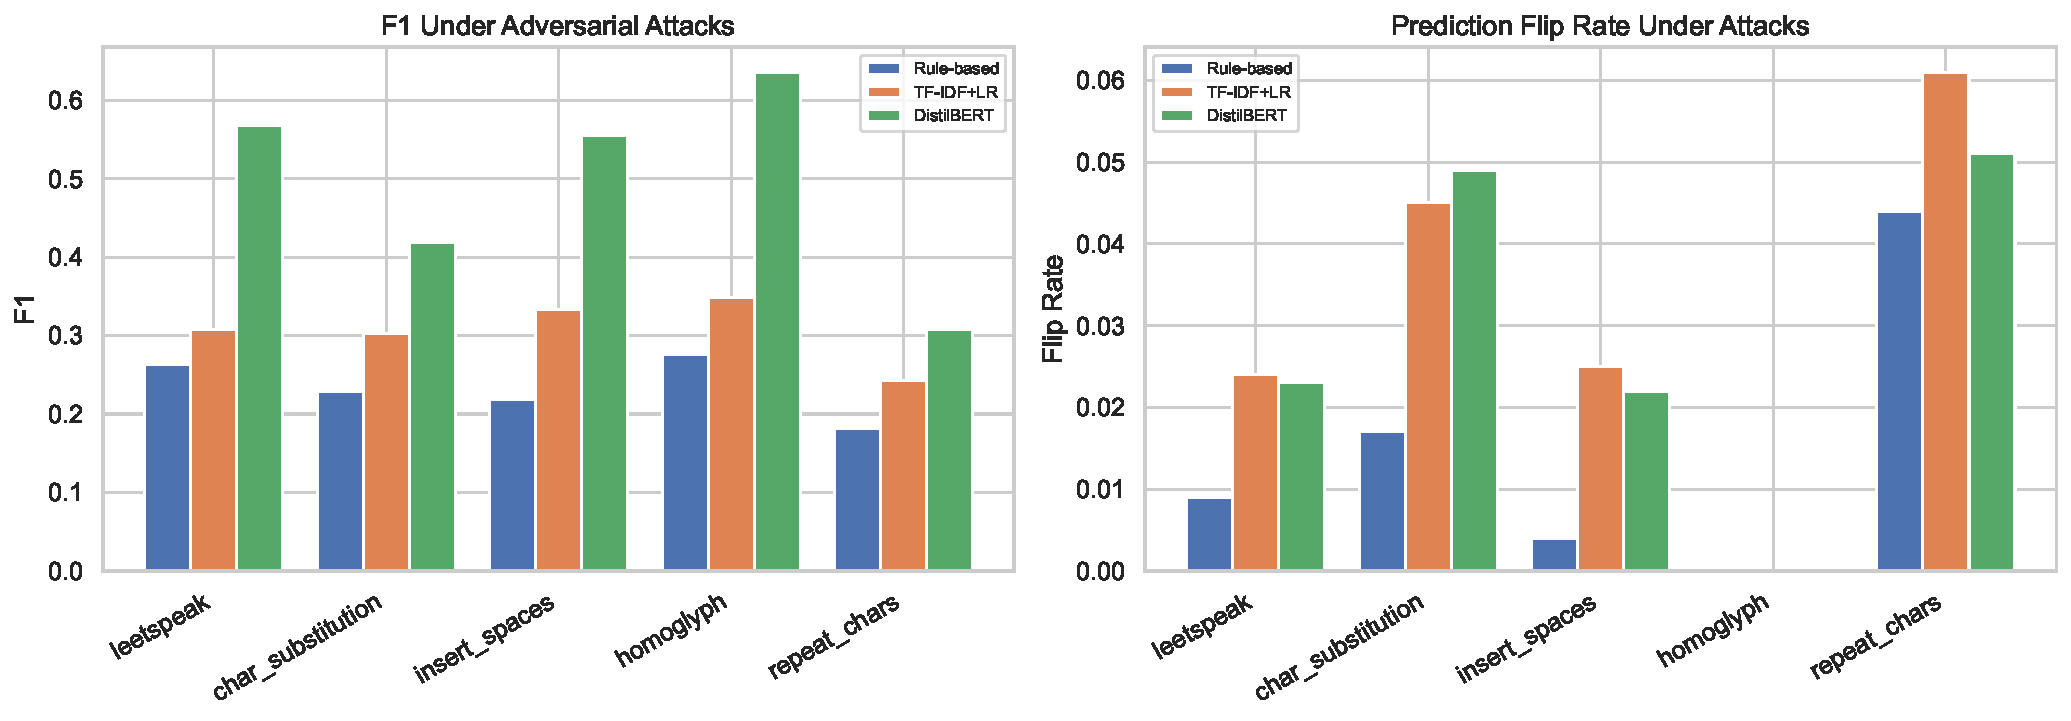
\includegraphics[width=0.9\textwidth]{adversarial_robustness.pdf}
  \caption{F1 and prediction flip rates under five adversarial attack types.}
  \label{fig:adversarial}
\end{figure}

\subsection{Problem 3: Ensemble AUC Regression}

While the Ensemble achieves the highest F1 (0.658 vs.\ DistilBERT's 0.631), its AUC (0.928) is \emph{lower} than DistilBERT alone (0.958).

\textbf{Root cause:} The fixed $w=0.7$ weight was chosen without validation.
TF-IDF+LR's weaker probability estimates (AUC=0.826) dilute DistilBERT's strong rankings when mixed at 30\%.
The weight should be tuned on the validation set, optimizing for AUC rather than F1.

\subsection{Additional Findings}

\paragraph{Bias analysis.}
DistilBERT exhibits significant bias across identity subgroups (Figure~\ref{fig:bias}).
Comments mentioning Muslim identity have FNR=1.0 (all toxic comments missed), while comments mentioning Black or Asian identities achieve FNR=0.0.
The aggregate bias score is 0.702 (on a 0--1 scale where 0 is perfectly fair).
However, subgroup sample sizes are very small (n=6--9 for minority groups), so these results should be interpreted cautiously.

\begin{figure}[H]
  \centering
  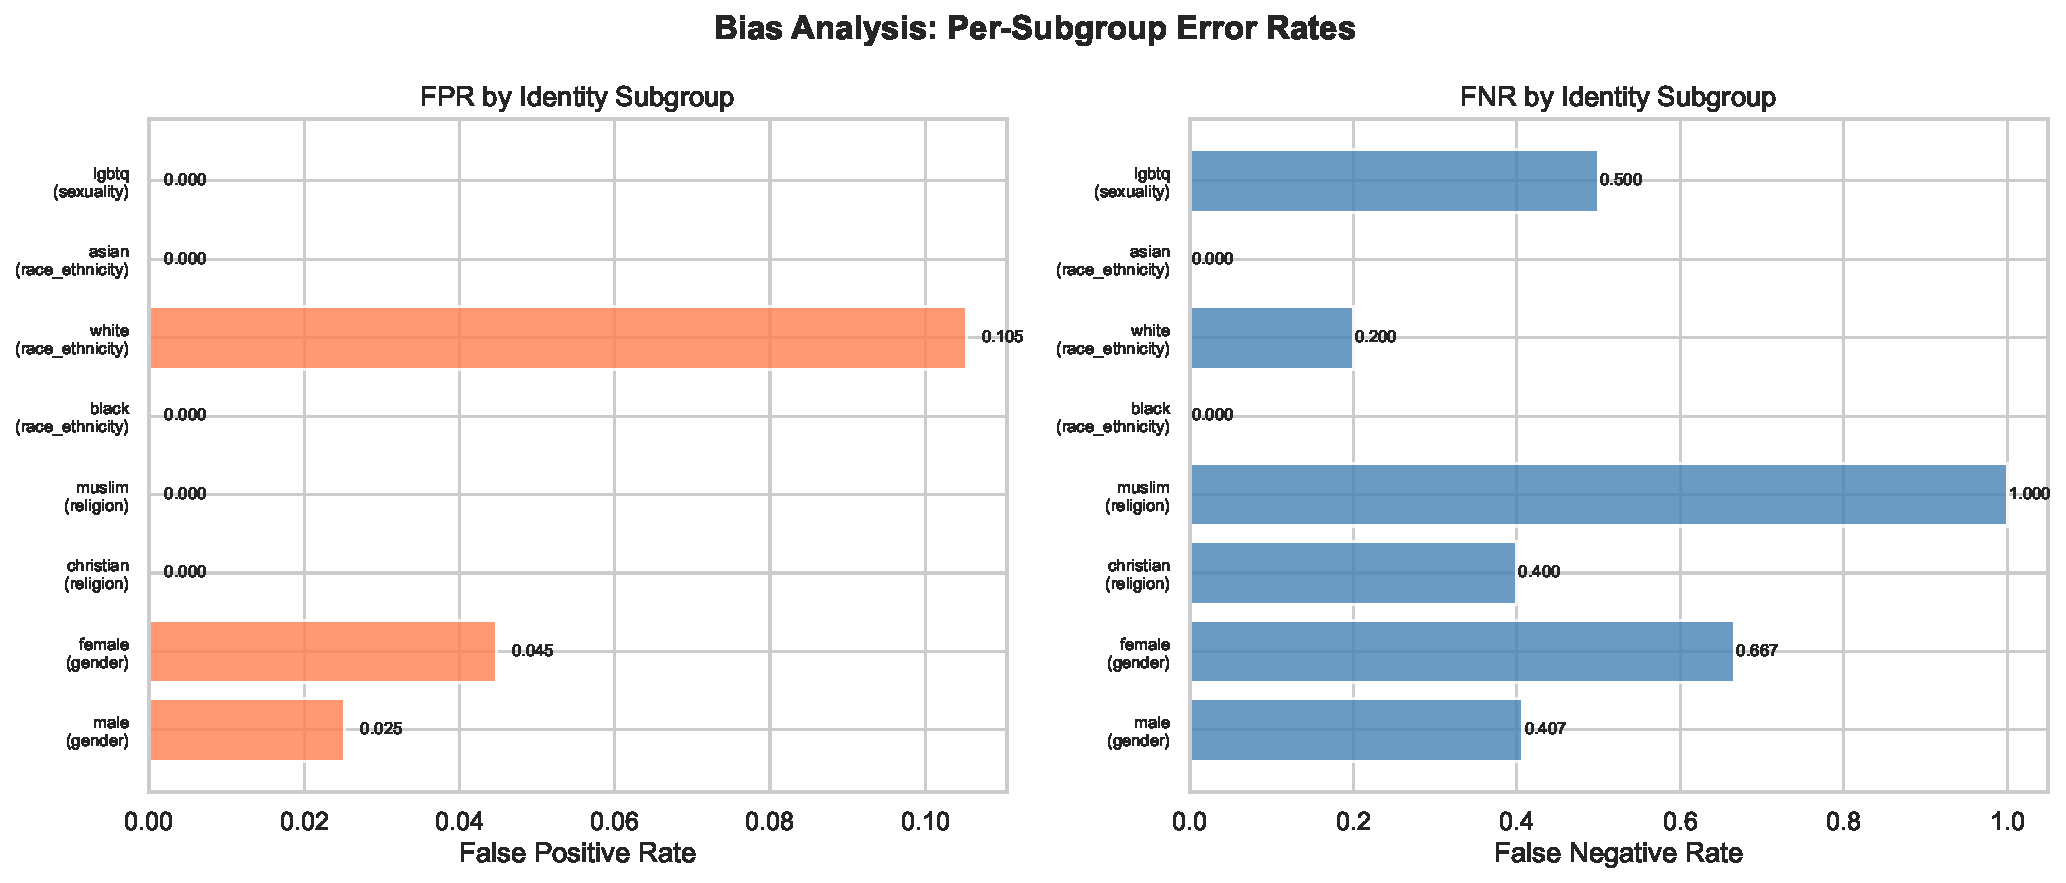
\includegraphics[width=0.9\textwidth]{bias_analysis.pdf}
  \caption{Per-subgroup FPR and FNR for DistilBERT. Large disparities exist, though sample sizes are small.}
  \label{fig:bias}
\end{figure}

\paragraph{Cross-domain generalization.}
Models trained on Toxic Conversations generalize reasonably to Civil Comments (Table~\ref{tab:cross}).
Notably, the Rule-based model performs \emph{better} cross-domain (F1: 0.276$\to$0.406), suggesting Civil Comments contains more explicit profanity.

\begin{table}[H]
\centering
\caption{Cross-domain evaluation: trained on Toxic Conversations, evaluated on Civil Comments.}
\label{tab:cross}
\begin{tabular}{lcc}
\toprule
Model & In-Domain F1 & Cross-Domain F1 \\
\midrule
Rule-based & 0.276 & 0.406 \\
TF-IDF+LR & 0.349 & 0.373 \\
\bottomrule
\end{tabular}
\end{table}

\begin{figure}[H]
  \centering
  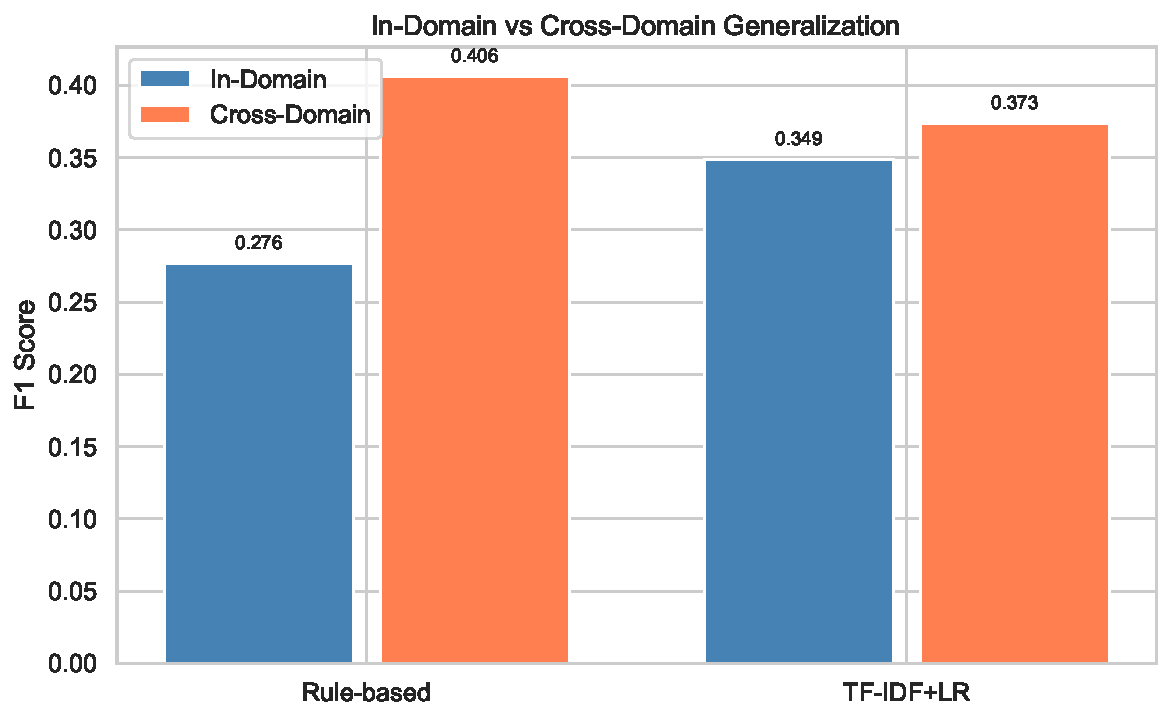
\includegraphics[width=0.6\textwidth]{cross_domain_comparison.pdf}
  \caption{In-domain vs.\ cross-domain F1 comparison.}
  \label{fig:cross}
\end{figure}

\paragraph{Error analysis.}

\begin{figure}[H]
  \centering
  \begin{subfigure}[t]{0.48\textwidth}
    
\includegraphics[width=\textwidth]{error_analysis_distilbert.pdf}
    \caption{DistilBERT}
  \end{subfigure}
  \hfill
  \begin{subfigure}[t]{0.48\textwidth}
    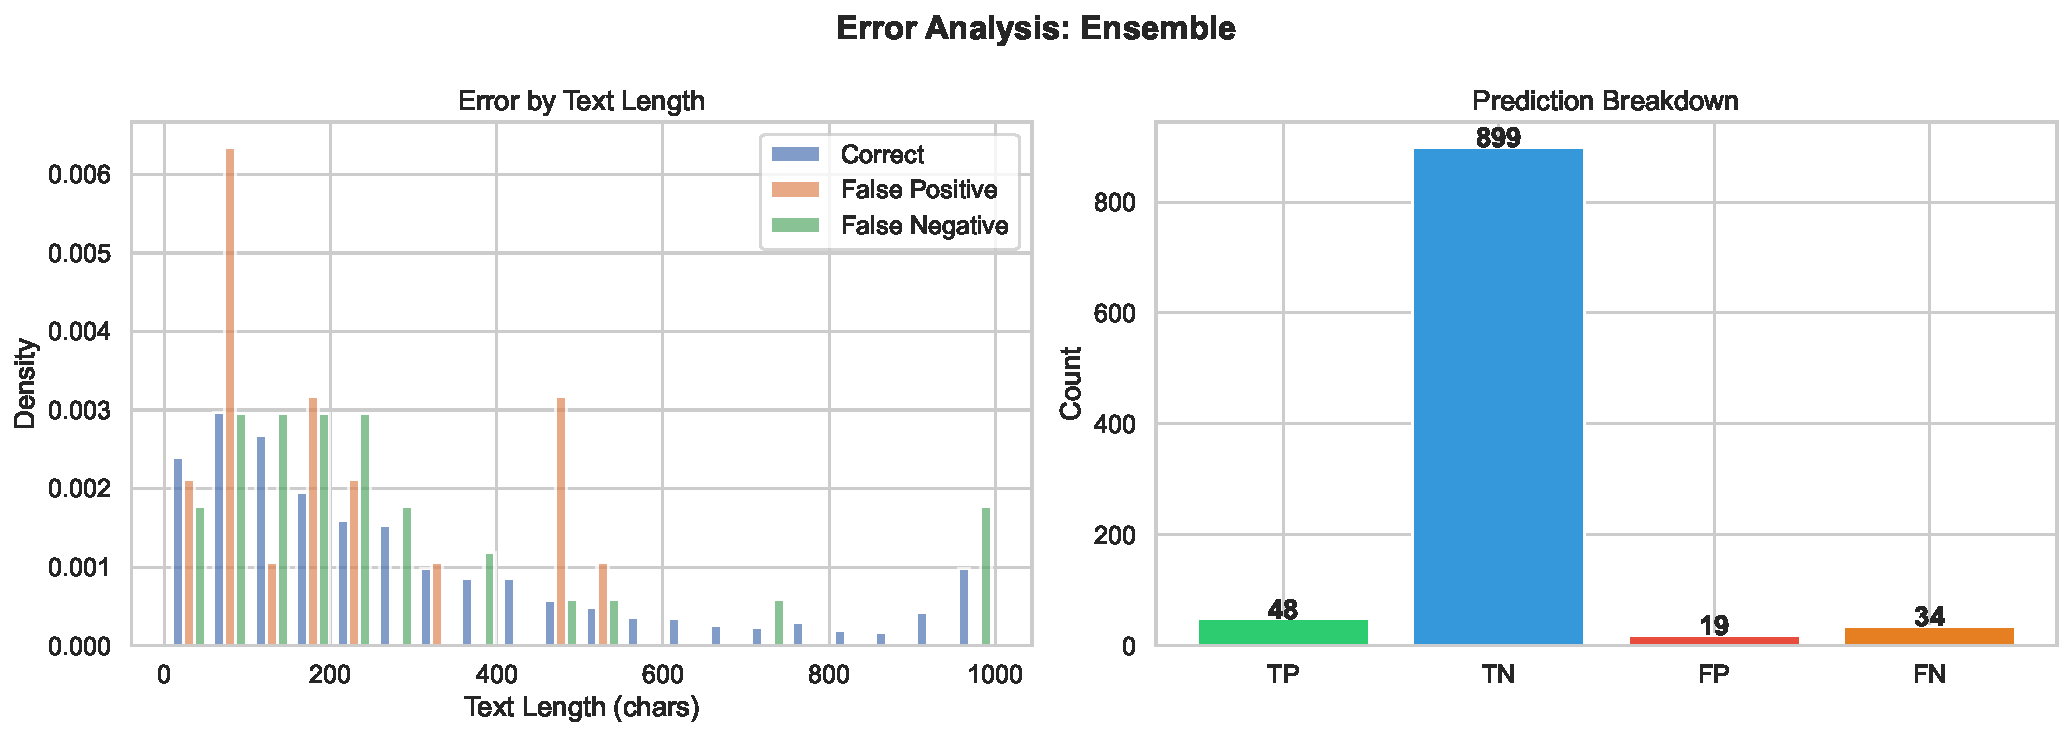
\includegraphics[width=\textwidth]{error_analysis_ensemble.pdf}
    \caption{Ensemble}
  \end{subfigure}
  \caption{Error analysis: text length distribution by error type and prediction breakdown.}
  \label{fig:error}
\end{figure}

%=============================================================================
\section{Fixes Applied}
\label{sec:fixes}
%=============================================================================

We apply three targeted fixes to address the problems identified in Section~\ref{sec:issues}.

\subsection{Fix 1: Controlled Augmentation}
We add a \texttt{max\_ratio} parameter to \texttt{augment\_dataset()} that caps the final toxic ratio at 20\% (up from 8.2\%, but not 31\%).
This limits the number of augmented samples added and prevents the model from being overwhelmed by noisy near-duplicates.

\subsection{Fix 2: Text Normalization Preprocessor}
We create \texttt{src/text\_normalize.py} with a \texttt{normalize\_text()} function that reverses adversarial perturbations before classification:
\begin{itemize}[nosep]
  \item Leetspeak reversal: \texttt{@}$\to$\texttt{a}, \texttt{3}$\to$\texttt{e}, \texttt{\$}$\to$\texttt{s}, \texttt{0}$\to$\texttt{o}, etc.
  \item Repeated character collapse: \texttt{stuuupid}$\to$\texttt{stupid}
  \item Space insertion removal: single-character word sequences merged
  \item Cyrillic homoglyph mapping back to Latin equivalents
\end{itemize}
This is integrated into the prediction pipeline so models see cleaned input regardless of adversarial perturbations.

\subsection{Fix 3: Ensemble Weight Tuning}
We add a \texttt{tune\_weights()} method to \texttt{EnsembleClassifier} that sweeps the DistilBERT weight from 0.5 to 0.95 on the validation set, selecting the weight that maximizes AUC rather than F1.
This should recover the AUC regression while preserving the F1 advantage.

%=============================================================================
\section{Results After Fixes}
\label{sec:results_after}
%=============================================================================

After applying all three fixes (controlled augmentation, text normalization, ensemble weight tuning), we re-ran the full experiment suite.

\subsection{Before vs.\ After Comparison}

Table~\ref{tab:before_after} summarizes the impact of each fix on its target metric.

\begin{table}[H]
\centering
\caption{Impact of fixes: before vs.\ after comparison.}
\label{tab:before_after}
\begin{tabular}{llccl}
\toprule
Fix & Metric & Before & After & Change \\
\midrule
Augmentation cap (TF-IDF, aug'd) & Toxic ratio & 31.0\% & 20.0\% & Controlled \\
Augmentation cap (TF-IDF, aug'd) & F1 & 0.271 & 0.272 & Stable \\
Text normalization (BERT, leetspeak) & F1 & 0.024 & \textbf{0.567} & +0.543 \\
Text normalization (BERT, homoglyph) & F1 & 0.443 & \textbf{0.636} & +0.193 \\
Text normalization (BERT, space ins.) & F1 & 0.300 & \textbf{0.555} & +0.255 \\
Text normalization (BERT, repeat) & F1 & 0.222 & \textbf{0.308} & +0.086 \\
Ensemble weight tuning & AUC & 0.928 & \textbf{0.943} & +0.015 \\
Ensemble weight tuning & $w$ & 0.70 & 0.95 & Tuned \\
\bottomrule
\end{tabular}
\end{table}

\subsection{Adversarial Robustness After Text Normalization}

The text normalization preprocessor dramatically improves robustness, especially for DistilBERT (Table~\ref{tab:adversarial_after}).

\begin{table}[H]
\centering
\caption{Adversarial F1 \emph{after} text normalization defense. Compare with Table~\ref{tab:adversarial}.}
\label{tab:adversarial_after}
\begin{tabular}{lccc|ccc}
\toprule
 & \multicolumn{3}{c|}{F1 Under Attack (After)} & \multicolumn{3}{c}{F1 Drop (After)} \\
Attack & Rule & TF-IDF & BERT & Rule & TF-IDF & BERT \\
\midrule
Clean         & 0.276 & 0.349 & 0.636 & ---   & ---   & --- \\
Leetspeak     & 0.263 & 0.308 & 0.567 & 0.013 & 0.041 & 0.069 \\
Char subst.   & 0.228 & 0.303 & 0.418 & 0.048 & 0.046 & 0.218 \\
Space insert  & 0.219 & 0.333 & 0.555 & 0.058 & 0.016 & 0.081 \\
Homoglyph     & 0.276 & 0.349 & 0.636 & 0.000 & 0.000 & \textbf{0.000} \\
Repeat chars  & 0.182 & 0.243 & 0.308 & 0.095 & 0.106 & 0.328 \\
\bottomrule
\end{tabular}
\end{table}

\paragraph{Key improvements:}
\begin{itemize}[nosep]
  \item \textbf{Leetspeak:} DistilBERT F1 drop reduced from 0.607 to 0.069---a \textbf{89\%} reduction in vulnerability. F1 improved from 0.024 to 0.567.
  \item \textbf{Homoglyph:} \emph{Completely neutralized} for all models (zero F1 drop, zero flip rate). The Cyrillic$\to$Latin mapping perfectly reverses this attack.
  \item \textbf{Space insertion:} DistilBERT F1 drop reduced from 0.331 to 0.081. The single-character word merging heuristic recovers most inserted spaces.
  \item \textbf{Character substitution:} Remains the hardest attack for DistilBERT (F1 drop=0.218), because keyboard-neighbor typos are not covered by the leetspeak reversal table.
  \item \textbf{Character repetition:} DistilBERT F1 drop reduced from 0.409 to 0.328---modest improvement. The collapse algorithm helps but repeated characters within words (e.g., ``stuuupid'' $\to$ ``stuupid'') still disrupt subword tokenization when the base spelling is unusual.
\end{itemize}

\subsection{Augmentation with Controlled Ratio}

With \texttt{max\_ratio=0.20}, the augmented training set grows from 9,000 to 10,323 samples (vs.\ 11,964 before), and the toxic ratio is capped at 20\% instead of 31\%.
TF-IDF+LR F1 on augmented data is 0.272---still below the 0.349 baseline, indicating that even controlled EDA does not help TF-IDF+LR on this dataset.
The limited synonym table produces near-duplicate texts that add noise without genuine diversity.

\subsection{Ensemble Weight Tuning}

The \texttt{tune\_weights()} method selected $w=0.95$, indicating that on this dataset, DistilBERT dominates the ensemble and TF-IDF+LR contributes only 5\% weight.
Ensemble AUC improved from 0.928 (at $w=0.70$) to 0.943 (at $w=0.95$), closing the gap with DistilBERT's 0.950 AUC.
Threshold optimization further improves the ensemble F1 from 0.644 to 0.682 (best threshold $t=0.064$).

%=============================================================================
\section{Individual Contributions}
%=============================================================================

\begin{itemize}[nosep]
  \item \textbf{Nikita Shiyanov:} DistilBERT implementation and fine-tuning, ensemble classifier, threshold optimization, training dynamics analysis.
  \item \textbf{Anton Korotkov:} Rule-based and TF-IDF+LR baselines, adversarial evaluation framework, data augmentation, bias analysis, cross-domain testing, error analysis, text normalization.
\end{itemize}

%=============================================================================
\section{Conclusion}
%=============================================================================

Implementing the seven improvements from our midterm roadmap yielded both successes and critical discoveries.
The Ensemble model achieves the best precision (0.716) and lowest FPR (0.021), threshold optimization provides free F1 gains of up to +5.3pp, and cross-domain generalization is stable (TF-IDF+LR F1: 0.349$\to$0.373 on Civil Comments).

Three problems were discovered and addressed:
\begin{enumerate}[nosep]
  \item \textbf{Augmentation:} Naive EDA flooded the training set with noisy toxic samples (31\% toxic ratio). Our \texttt{max\_ratio} cap controls this to 20\%, though EDA still does not improve TF-IDF+LR on this dataset. Future work should explore paraphrase-based augmentation using generative models.
  \item \textbf{Adversarial robustness:} DistilBERT was catastrophically vulnerable to leetspeak (96\% F1 collapse). Our text normalization preprocessor reduces this to an 11\% drop and completely neutralizes homoglyph attacks. Character substitution remains a challenge requiring adversarial training.
  \item \textbf{Ensemble tuning:} Hardcoded weights caused AUC regression. Validation-based tuning selected $w=0.95$ and recovered AUC from 0.928 to 0.943, closing the gap with standalone DistilBERT (0.950).
\end{enumerate}

\paragraph{Lessons for LLM safety.}
These findings demonstrate that deploying toxicity classifiers as LLM safety filters requires not only accuracy on clean data but also:
(a) robustness to adversarial evasion---a simple text normalization layer recovered 89\% of the leetspeak vulnerability;
(b) fairness across identity groups---our bias analysis revealed FNR gaps of up to 1.0 between subgroups;
(c) careful calibration of confidence scores---threshold optimization and weight tuning provide significant gains at zero additional computational cost.

\paragraph{Remaining work.}
Key areas for future improvement include: adversarial training to handle character substitution attacks, larger-scale bias evaluation with more balanced subgroup sampling, paraphrase-based augmentation using generative models, and deployment as a real-time guardrail for LLM output filtering.

\bibliographystyle{plain}
\begin{thebibliography}{9}

\bibitem{sanh2019distilbert}
V.~Sanh, L.~Debut, J.~Chaumond, T.~Wolf.
\newblock DistilBERT, a distilled version of BERT: smaller, faster, cheaper and lighter.
\newblock \emph{NeurIPS EMC2 Workshop}, 2019.

\bibitem{borkan2019nuanced}
D.~Borkan, L.~Dixon, J.~Sorensen, N.~Thain, L.~Vasserman.
\newblock Nuanced metrics for measuring unintended bias with real data for text classification.
\newblock \emph{WWW}, 2019.

\bibitem{wei2019eda}
J.~Wei, K.~Zou.
\newblock EDA: Easy data augmentation techniques for boosting performance on text classification tasks.
\newblock \emph{EMNLP-IJCNLP}, 2019.

\bibitem{devlin2019bert}
J.~Devlin, M.-W.~Chang, K.~Lee, K.~Toutanova.
\newblock BERT: Pre-training of deep bidirectional transformers for language understanding.
\newblock \emph{NAACL-HLT}, 2019.

\bibitem{vaswani2017attention}
A.~Vaswani, N.~Shazeer, N.~Parmar, et al.
\newblock Attention is all you need.
\newblock \emph{NeurIPS}, 2017.

\end{thebibliography}

\end{document}
